\chapter{Étude du contexte}

  \lettrine[nindent=0em,lines=3]{L}e but de ce projet sera dans un premier temps
  de mettre en place une infrastructure de compilation, de test et d'exécution
  d'un noyau Linux. La seconde partie du projet sera de comprendre comment
  fonctionne le noyau Linux au niveau de la mémoire, notamment pour la gestion
  des pages (emplacement, taille), et au niveau des processeurs pour le
  placement des threads et le parallélisme. Ensuite, il faudra se plonger dans
  la lecture du code et sa modification aux endroits adéquats en utilisant des
  technologies comme IBS où les hardware counters pour obtenir des informations
  précises sur la gestion des points évoqués ci-dessus. Enfin, pour tester ce
  noyau avec nos modifications, nous utiliserons la machine virtuelle et gdb
  pour le débugage.
  %% TODO: changer débugage par autre chose

  \section{Infrastructure}
    \subsection{Machine virtuelle}
        Dans cette partie, nous allons détailler l'infrastructure dont nous
        disposons et celle que nous avons mise en place pour ce projet. Notre avons
        à notre disposition une machine AMD Opteron 6172 composée de quatre
        processeurs à douze coeurs chacun cadencés à 2,1GHz et répartis en 8 noeuds
        avec 32G de mémoire vive. (cf. Figure 2.1)

        %% TODO: vérifier l'archi à la main (méga chaud et méga long)

        %% node   0   1   2   3   4   5   6   7 
        %%   0:  10  16  16  22  16  22  16  22 
        %%   1:  16  10  16  22  22  16  22  16 
        %%   2:  16  16  10  16  16  16  16  22 
        %%   3:  22  22  16  10  16  16  22  16 
        %%   4:  16  22  16  16  10  16  16  16 
        %%   5:  22  16  16  16  16  10  22  22 
        %%   6:  16  22  16  22  16  22  10  16 
        %%   7:  22  16  22  16  16  22  16  10

        \begin{figure}[!ht]
          \centering
          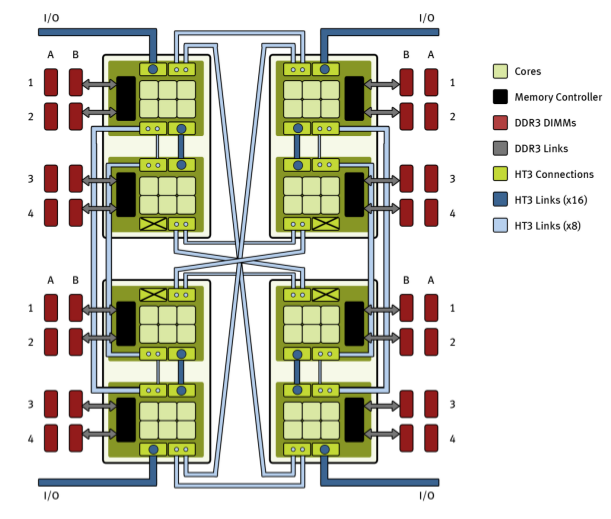
\includegraphics[scale=0.55]{img/numa_arch_details.png}
          \caption{Topologie de la machine 6172}
          \label{f:numa_topology}
        \end{figure}

        Sur cette machine, nous avons utilisé l'Hyperviseur qemu, avec son extension
        kvm pour afin d'optimiser l'émulation. Afin d'améliorer encore plus cette
        dernière, nous avons utilisé le logiciel virt-manager qui détecte
        automatiquement la configuration matérielle de machine hôte et configure la
        machine virtuelle en conséquence. Cette configuration est à notre avis très
        réaliste puisqu'elle est capable d'activer/désactiver des options CPU comme
        la gestion d'IBS où l'hypervision. Un des autres avantage de virt-manager
        est que l'on peut sauvegarder la configuration dans un fichier, et pouvoir
        ainsi l'exporter facilement.

        Nous avons installé une machine virtuelle classique (Debian GNU/Linux), qui
        nous permettra par la suite de fournir à notre noyau compilé une
        architecture de base pour se lancer. En effet, la compilation du noyau se
        fera directement sur l'Opteron, mais le lancement et les tests se feront via
        l'hyperviseur. Afin que le noyau puisse se lancer et avoir une base, nous
        avons installé une première VM, donc nous récupérerons la configuration du
        noyau pour la compilation.

    \subsection{GDB mode remote}

        Les modifications apportées au noyau doivent être controlées en cas d'erreur 
        dans le code pendant la periode de développement. Pour ce faire nous allons 
        utiliser gdb, le debugger sous licence libre distribué par le groupe du 
        projet GNU. L'utilisation que nous allons faire sur gdb n'est pas une 
        utilisation commune comme cela se fait sur un programme classique car
        dans notre cas, étant donné que c'est le noyau lui même qui est en train de se
        charger, il n'est pas possible d'executer un programme tel que gdb sur la 
        machine. Pour pouvoir l'utiliser et débugger le noyau modifié, nous allons
        utiliser une option de gdb qui va nous permettre une execution controlée
        du noyau, plus précisément le control de breakpoints. \\

        Effectivement, le mode remote de gdb va nous permettre de mettre en place 
        une telle configuration. Et il se trouve que qemu va fournir également 
        une option d'interface entre une VM et une machine distante.
        Ainsi, dans notre cas, il va falloir lancer premièrement qemu avec l'option
        \og -s -S\fg qui va se charger de fournir le \og gdb stub\fg nécéssaire a la 
        connexion distante de gdb en mode remote, qemu se lance alors, sans lancer 
        la machine virtuelle, en attente d'une connexion sur le port 1234 
        (par defaut) de la machine qui execute la machine virtuelle.
        Ensuite il nous faut donc lancer gdb en lui fournissant l'image du noyau 
        Linux compilé afin que celui-ci puisse charger la table des symboles 
        pour pouvoir placer les breakpoints :
        \begin{lstlisting}
        gdb ./vmlinux
        \end{lstlisting}
        Ensuite nous lançons la connexion sur le gdb stub de qemu (ici nous lançons 
        les deux programme sur la même machine, la connexion se fait donc en local) :
        \begin{lstlisting}
        (gdb) target remote localhost:1234
        \end{lstlisting}
        Maintenant nous avons connecté gdb à qemu et nous pouvons commencer le 
        debuggage du noyau (à distance) en placant des breakpoints là où il y en a
        besoin.

  \section{La gestion de la mémoire}

    Sur une architecture NUMA, les performances des applications dépendent
    fortement du placement mémoire. Ce placement est contrôlé par le système
    d'exploitation via le mécanisme de pagination offert par le matériel. Le
    mécanisme de pagination permet d'offrir une vue virtualisée de la
    mémoire. Lorsque la pagination est activée, les instructions d'accès à la
    mémoire manipulent des adresses mémoire dites virtuelles. La MMU (Memory
    Management Unit) d'un coeur convertit alors l'adresse mémoire virtuelle en
    adresse mémoire physique avant d'effectuer l'accès mémoire. Pour effectuer
    cette conversion, la MMU utilise une table des pages dont l'adresse est
    stockée dans un des registre du coeur. Cette table associe des plages
    d'adresses virtuelles de taille fixe à des plages d'adresses physiques de
    même taille. Dans le contexte de la pagination, cette plage d'adresse fixe
    est appelée une page.

    Le système d'exploitation maintient une table des pages par processus, donc
    partagée par les threads du processus. Le système s'occupe de la remplir et
    de la modifier en fonction des besoins du processus. Techniquement,
    lorsqu'un processus alloue un espace mémoire à bas niveau (fonction mmap),
    le système lui donne une autorisation d'accès à une plage d'adresse
    virtuelle appelé XX\footnote{TODO} mais n'y associe pas encore de page
    physique. Elles sont associées aux pages virtuelles de façon paresseuse : à
    chaque fois que le processus accède à une page virtuelle qui n'est pas
    encore présente dans la table des pages, le processeur déclenche une faute
    des pages. Cette faute est rattrapée par une fonction du système qui
    s'occupe alors de trouver une page physique libre pour l'associer à la page
    virtuelle ayant déclanché la faute.
  
    Sur une architecture NUMA, l'espace d'adressage physique est lui-même
    partitionné entre les noeuds NUMA. Les premières adresses physique sont
    associées au premier noeud, les suivantes au second etc\ldots Lorsque le
    système d'exploitation associe une page virtuelle à une page physique dans
    une table des pages, il choisit donc sur quel noeud les accès à la page
    virtuelle seront effectués en fonction de l'adresse de la page physique. Le
    système peut aussi choisir de migrer une page virtuelle d'un noeud vers un
    autre en copiant la page physique vers un autre noeud et en mettant à jour
    la table des pages.

    Pour effectuer un placement mémoire optimisant les performances des
    processus, le système d'exploitation doit donc être capable de sélectionner
    sur quel noeud placer les pages virtuelles. Ce choix dépend directement du
    coeur sur lequel s'exécute le thread qui accède à la page, le but étant
    d'essayer de placer le thread et les pages auxquelles il accède sur le même
    noeud. La question devient donc, quels sont les threads qui demandent le
    plus d’accès mémoire et sur quels noeuds sont-ils placés?
    %% Une des mesures significatives lorsque l'on s'intéresse à la mémoire est
    %% le nombre de défaut de page, également appelé \og cache miss\fg ou \og
    %% CM\fg. Un défaut de page se produit lorsqu'un processus demande à la
    %% mémoire une ressource, mais que celle-ci ne s'y trouve pas. La mémoire
    %% envoie alors le signal \og miss\fg au processeur, va charger la ressource
    %% et lui renvoi.  Le mapping de la mémoire est un problème en soit quelque
    %% soit le système d'exploitation et l'architecture, mais il se révèle très
    %% complexe lorsque l'on se retrouve avec une architecture NUMA. Où doit-on
    %% placer les objets en mémoire ? Où plutot, dans quel noeud doit-on les
    %% placer ? Tout dépend du noeud démandant le plus d'accès à ces objets. La
    %% question devient donc, quels sont les processus qui demandent le plus
    %% d'accès mémoire et sur quels noeuds sont-ils placés ?
    Si les accès sont distants, les noeuds sont-ils très éloignés ?
    Engendrent-ils une congestion dans les interconnexions ? Si oui, quel est le
    coût d'un déplacement de page mémoire ? Toutes ces questions et tous ces
    paramètres sont à prendre en compte lors des (dé)placements en mémoire des
    données.

    Prenons l'exemple d'une application générant énormément d'accès mémoire. Le
    nombre de cache miss peut être très élevé si les données sont réparties
    équitablement sur différents noeuds, ou au contraire placées sur un seul
    noeud distant, avec un bus d'échange plus ou moins rapide avec le noeud
    demandant les données. Et là encore, tout dépend de l'application utilisant
    ces données. Certaines applications fonctionneront mieux si les données sont
    réparties équitablement sur les noeuds, et au contraire certaine verront
    leur performances largement dégradées.

    Une expérience illustrant ce phénomène a été réalisée l'année
    dernière\cite{Holistic2013}. L'équipe de recherche a \og stressé\fg une
    machine NUMA avec différentes applications plus où moins gourmande en
    ressource. La mémoire est soit gérée en \og First-Touch (F)\fg, c'est à dire
    que les données sont placées dans le premier noeud entrainant un cache miss,
    soit en \og interleaving (I)\fg, et dans ce cas les données sont réparties
    équitablement entre les noeuds. Voici les résultats qu'ils ont obtenus:

    \begin{figure}[!ht]
      \centering
      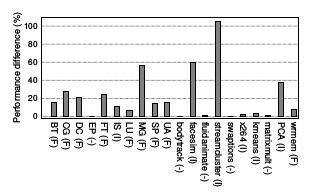
\includegraphics[scale=0.80]{img/numa_memory_policy}
      \caption{Différences de performances en fonction de la politique de
        placement en mémoire sur une architecture NUMA (\textit{First-Touch ou Interleaving})}
    \end{figure}

    On voit que les résultats sont largement différents selon les applications
    et la politique de gestion. Ainsi, une de nos approches sera d'observer le
    fonctionnement de la mémoire selon ces différentes applications, étudier les
    défaut de pages, comprendre pourquoi certaines fonctionnent mieux que
    d'autres, et essayer d'identifier des \og familles d'applications\fg ayant
    comme trait commun leur comportement vis-à-vis de la mémoire.
    
  \section{Communication entre threads}
    
    Un autre challenge quant à l'optimisation de performance sur architecture 
    NUMA sont les communications et les echanges de données qui peuvent s'effectuer 
    entre 
    plusieurs threads de façon simultanée. En effet nous allons devoir fournir un 
    moyen
    de mesurer ces communications afin que notre noyau 
    puisse utiliser une politique de placement des thread qui leur permette de 
    se retrouver les plus proches les uns des autres, de cette façon, leurs échanges 
    ne se feront (idéalement) que sur un seul et même noeud. Nous effectuerons donc
    une grande partie de ce monitoring sur les échanges menés par des tubes.

  \section{But à terme}

    Ce projet PSAR a pour but d'être ensuite intégré au sein d'un projet de plus
     grande 
    envergure, en effet, le but ici étant de fournir des informations et des outils
    de monitoring sur différentes activités du noyau. Cela pour permettre ensuite 
    l'étude de différents algorithmes des placement mémoires au sein du noyau Linux
    qui permettra d'optimiser les performances des architectures NUMA (
    algorithmes de \og ressorts\fg).
